%----------------------------%
%----    preamble.tex    ----%
%----------------------------%

\usepackage{booktabs}
\usepackage{amsthm}
\makeatletter
\def\thm@space@setup{%
  \thm@preskip=8pt plus 2pt minus 4pt
  \thm@postskip=\thm@preskip
}
\makeatother

%----    layout    ----%

% change margins
\usepackage[outer = 105pt, inner = 85pt]{geometry}
\usepackage{afterpage}
\voffset 5pt
\headsep 29pt
\footskip 35pt
\textheight 590pt
\usepackage{layout}% http://ctan.org/pkg/layouts

% caption
\usepackage[labelfont=bf]{caption}


%---- page numbers header and footer
\usepackage{xcolor}

\definecolor{ctcolorgraylight}{RGB}{153, 153, 153}
\definecolor{ctcolorgray}{RGB}{120, 120, 120}

\usepackage{fancyhdr}
\usepackage[fit]{truncate}

% Redefine the plain page style
\fancypagestyle{plain}{%
  \fancyhf{}%
  \fancyfoot[LE,RO]{\textcolor{ctcolorgray}{\thepage}}
  \renewcommand{\headrulewidth}{0pt}% Line at the header invisible
}

% fancy style
\fancypagestyle{myfancy}{%
  \fancyhf{}
  \fancyhead[LE]{\footnotesize\textit{\nouppercase{\truncate{0.98\headwidth}{\textcolor{ctcolorgray}{\rightmark}}}}}
  \fancyhead[RO]{\footnotesize\textit{\truncate{0.98\headwidth}{\textcolor{ctcolorgray}{\leftmark}}}}
  \fancyfoot[LE,RO]{\textcolor{ctcolorgray}{\thepage}}
  \renewcommand{\headrulewidth}{1.5pt}
  \renewcommand{\headrule}{\hbox to\headwidth{%
      \color{ctcolorgraylight}\leaders\hrule height \headrulewidth\hfill}}
}

% part page style
\newcommand{\cpart}[1]{
\cleardoublepage
\stepcounter{part}
\pagestyle{empty}
\begin{flushright}
  \vspace*{2.5cm}
  {\fontfamily{pnc}\fontsize{75}{80}\selectfont%
   \textcolor{ctcolorgraylight}{\textbf{Part \thepart}}\par}%
  \vspace*{1cm}
  {\Huge\textbf{#1}}%
  \end{flushright}
\addcontentsline{toc}{part}{Part \thepart\hspace{1em}#1}
\cleardoublepage
\pagestyle{plain}
}

\usepackage{titletoc}
\titlecontents{part}[0pt]{\bfseries\protect\addvspace{20pt}\titlerule\addvspace{.7ex}}%
{}{}%% numbered/numberless formatting
{}%% to be replaced with {} if you don't want any page number for parts
[\addvspace{0.7ex}\titlerule\addvspace{1.5ex}]

%---- chapter title
\usepackage[newcentury]{quotchap}

\makeatletter
\renewcommand*{\chapnumfont}{%
  \usefont{T1}{\@defaultcnfont}{b}{n}\fontsize{120}{150}\selectfont% Default: 100/130
  \color{chaptergrey}%
}
\makeatother


%----    define infoboxes    ----%
\usepackage[skins, most]{tcolorbox}

% colors
\definecolor{background}{HTML}{fcfcfc}
\definecolor{tip-text}{HTML}{e7b002}
\definecolor{tip-line}{HTML}{fdce38}
\definecolor{warning-text}{HTML}{b06336}
\definecolor{warning-line}{HTML}{c97d50}
\definecolor{deffun-text}{HTML}{0b797e}
\definecolor{deffun-line}{HTML}{6CC2C9}
\definecolor{design-text}{HTML}{7c972e}
\definecolor{design-line}{HTML}{a7c84a}
\definecolor{trick-text}{HTML}{8c3031}
\definecolor{trick-line}{HTML}{A3595A}

\newtcolorbox{mybox}[1][black]{
  colback=background,
  coltext=black,
  colframe=#1,
  boxsep=5pt,
  arc=4pt,
  breakable}

% tip
\newenvironment{tip}[1][Title]
  {
  \setlength{\fboxsep}{1em}
  \begin{mybox}[tip-line]
    \raisebox{-.2\height}{
\includegraphics[height=.6cm]{assets/images/lightbulb.png}} \large \textcolor{tip-text}{Tip-Box: #1\\\vspace*{.5em}}\normalsize
    }
    {
  \end{mybox}
  }

% warnings
\newenvironment{warning}[1][Title]
  {
  \setlength{\fboxsep}{1em}
  \begin{mybox}[warning-line]
    \raisebox{-.2\height}{
\includegraphics[height=.6cm]{assets/images/gotcha.png}} \large \textcolor{warning-text}{Warning-Box: #1\\\vspace*{.5em}}\normalsize
    }
    {
  \end{mybox}
  }

% deffun
\newenvironment{deffun}[1][Title]
  {
  \setlength{\fboxsep}{1em}
  \begin{mybox}[deffun-line]
    \raisebox{-.2\height}{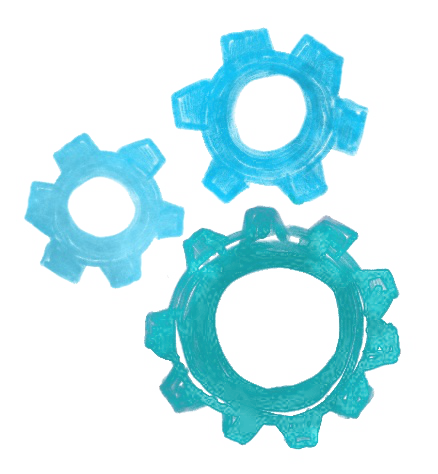
\includegraphics[height=.6cm]{assets/images/gears.png}} \large \textcolor{deffun-text}{Instructions-Box: #1\\\vspace*{.5em}}\normalsize
    }
    {
  \end{mybox}
  }

% doclinks
\newenvironment{doclinks}
  {
  \setlength{\fboxsep}{1em}
  \begin{mybox}[deffun-line]
    \raisebox{-.2\height}{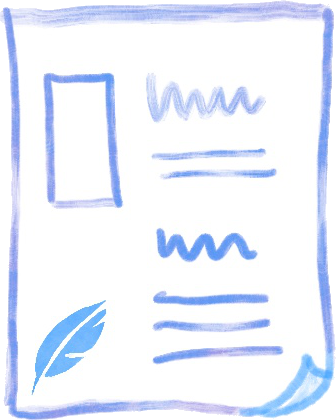
\includegraphics[height=.6cm]{assets/images/doc-links.png}} \large \textcolor{deffun-text}{Documentation-Box}\vspace*{.5em}\normalsize
    }
    {
  \end{mybox}
  }

% design
\newenvironment{design}[1][Title]
  {
  \setlength{\fboxsep}{1em}
  \begin{mybox}[design-line]
    \raisebox{-.2\height}{
\includegraphics[height=.6cm]{assets/images/design.png}} \large \textcolor{design-text}{Details-Box: #1\\\vspace*{.5em}}\normalsize
    }
    {
  \end{mybox}
  }

% trick
\newenvironment{trick}[1][Title]
  {
  \setlength{\fboxsep}{1em}
  \begin{mybox}[trick-line]
    \raisebox{-.2\height}{
\includegraphics[height=.6cm]{assets/images/hat.png}} \large \textcolor{trick-text}{Trick-Box: #1\\\vspace*{.5em}}\normalsize
    }
    {
  \end{mybox}
  }

%----    quote


\definecolor{block-gray}{gray}{0.95}


\newtcolorbox{line-left}{%
    colback=white,
    % grow to right by=-10mm,
    % grow to left by=-10mm,
    boxrule=0pt,
    boxsep=0pt,
    breakable,
    enhanced jigsaw,
    borderline west={2pt}{0pt}{gray},
    borderline north={0pt}{0pt}{white},
    borderline south={0pt}{0pt}{white},
    % title={#2\par},
    % colbacktitle={block-gray},
    % coltitle={black},
    % fonttitle={\large\bfseries},
    % attach title to upper={},
    % #1,
}

% \renewenvironment{quote}
%                {\begin{line-left}}
%                {\end{line-left}}

\renewenvironment{quote}
               {\list{}{\rightmargin\leftmargin}%
                \item\relax\begin{line-left}\setlength{\parskip}{1em}}
               {\end{line-left}\endlist}

%----    code-tex-*    ----%

\newenvironment{code-tex-bad}
  {\begingroup\definecolor{shadecolor}{RGB}{255, 189, 185}}
  {\endgroup}

\newenvironment{code-tex-good}
  {\begingroup\definecolor{shadecolor}{RGB}{224, 240, 227}}
  {\endgroup}

\newenvironment{code-tex-warn}
  {\begingroup\definecolor{shadecolor}{RGB}{249, 249, 154}}
  {\endgroup}


%----

\usepackage{hyperref}

